\documentclass[12pt]{article}
\usepackage[margin=1in]{geometry} 
\usepackage{amsmath,amsthm,amssymb,amsfonts}
\usepackage{listings}

\usepackage{graphicx}
\usepackage{subfig}
\newcommand{\N}{\mathbb{N}}
\newcommand{\Z}{\mathbb{Z}}
 
\newenvironment{problem}[2][Problem]{\begin{trivlist}
\item[\hskip \labelsep {\bfseries #1}\hskip \labelsep {\bfseries #2.}]}{\end{trivlist}}
%If you want to title your bold things something different just make another thing exactly like this but replace "problem" with the name of the thing you want, like theorem or lemma or whatever
 
\begin{document}
 
%\renewcommand{\qedsymbol}{\filledbox}
%Good resources for looking up how to do stuff:
%Binary operators: http://www.access2science.com/latex/Binary.html
%General help: http://en.wikibooks.org/wiki/LaTeX/Mathematics
%Or just google stuff
 
\title{Biomath 204 Homework 1}
\author{Benjamin Chu}
\maketitle
 
\begin{problem}{1}
Prove the Gauss-Markov theorem for $\beta_0$ in the following simple linear regression model:
$$Y_i = \beta_0 + \beta_1X_i + \epsilon_i,$$
assuming $E(\epsilon_i) = 0, Var(\epsilon_i') = \sigma^2, Cov(\epsilon_i, \epsilon_j) = 0.$
\end{problem}

\begin{proof}
In class we derived that $b_0 = \bar{Y} - b_1\bar{X}.$ To show $b_0$ is unbiased, note:

$$E(\bar{Y}) = \frac{1}{n} E(\sum_i Y_i) = \frac{1}{n}\sum_i [\beta_0 + \beta_1X_i] = \frac{1}{n} n \beta_0 + \frac{1}{n}\beta_1 \sum_i X_i = \beta_0 + \beta_1\bar{X}$$

On the other hand, $E(\beta_1 X_i) = \beta_1\bar{X},$ so 
$$E(b_0) = E(\bar{Y} - \beta_1X_i) = E(\bar{Y}) - E(\beta_1X_i) = \beta_0 + \beta_1\bar{X} - \beta_1\bar{X} = \beta_0.$$ 

To show linearity in $Y$, recall in lecture we showed $$b_1 = \sum_i k_iY_i, \quad k_i = \frac{(X_i - \bar{X})}{\sum_i (X_i - \bar{X})^2}.$$

Using this, we have 
\begin{equation}
\begin{split}
b_0 
&= \bar{Y} - b_1 \bar{X}\\
&= \bar{Y} - \big(\sum_i k_iY_i\big)\bar{X}\\
&= \frac{1}{n}\sum Y_i - \frac{1}{n}\sum_i k_iY_i \bar{X} n\\
&= \frac{1}{n}\sum\big[Y_i - k_iY_i\bar{X}n\big]\\
&= \sum Y_i \big(\frac{1}{n} - k_i\bar{X}\big) \\
&= \sum Y_i c_i
\end{split}
\end{equation}

Finally, to show min variance, let $\widetilde{b_0}$ be another estimator so that 
$$\widetilde{b_0} = \sum Y_ir_i$$

For some $r_i$. We need to show that $V(\widetilde{b_0}) \geq V(b_0).$ 
$$V(\widetilde{b_0}) = \sum V(Y_i)r_i^2 = \sigma^2 \sum r_i^2.$$
From here, following the strategy in lecture, define $d_i = r_i - c_i$, so that 
$$\sigma^2 \sum r_i^2 = \sigma^2 \sum (d_i + c_i)^2 = \sigma^2 \sum\Big[ d_i^2 + 2d_ic_i + c_i^2 \Big]$$

Because $d_i^2 \geq 0$, if we could show $d_ic_i = 0$, then we are done, because $V(b_0) = \sigma^2 \sum c_i^2$. To show this, do a bunch of algebra:
\begin{equation}
\begin{split}
\sum d_i c_i =\sum (r_i - c_i)c_i = \sum r_ic_i - \sum c_i^2\\ 
\end{split}
\end{equation}
Now because $\widetilde{b_0}$ is another estimator, the $r_i$'s must satisfy the following properties that $c_i$'s from $b_0$ satisfy:
$$\sum c_i = \sum(\frac{1}{n} - k_i \bar{X}) = 1-\bar{X}\sum k_i = 1 - 0 = 1$$
$$\sum c_ik_i = \sum (\frac{1}{n} - k_i \bar{X})k_i = \sum \frac{k_i}{n} - \bar{X}\sum k_i^2 = 0 - \frac{\bar{X}}{\sum(x-\bar{X})^2}$$
By these two, we can evaluate the two terms from eq(2) as follows:
$$\sum r_i c_i = \sum r_i(1/n - k_i \bar{X}) = \frac{1}{n}\sum r_i - \bar{X} \sum r_ik_i = 1 + \frac{\bar{X}}{\sum(X-\bar{X})^2}$$

$$\sum c_i^2 = \sum (\frac{1}{n} - k_i \bar{X})^2 = \sum (\frac{1}{n^2} - \frac{2k_i\bar{X}}{n} + \bar{X}^2k_i^2) = \frac{1}{n} + \frac{\bar{X}^2}{\sum(x-\bar{x})^2}$$

Now putting everything together:
$$\sum r_ic_i - \sum c_i^2 = \frac{1}{n} + \frac{\bar{X}^2}{\sum(X-\bar{X})^2} - \frac{1}{n} - \frac{\bar{X}^2}{\sum(X-\bar{X})^2} = 0$$
Therefore $V(b_0) \leq V(\widetilde{b_0})$ and we have proven the gauss-markov theorem completely.
\end{proof}

\begin{problem}{2}
Given $b_0, b_1$ are least-square estimators for the above regression model, show that the point $(\bar{X}, \bar{Y})$ always falls on the line $Y_i = b_0 + b_1X_i.$
\end{problem}

\begin{proof}
Intuitively, if we have a line that we know best estimates a set of data, then that line should be placed so that the sum of squared error is minimized. As in any refression, $X_i$ are the inputs (observed) and $Y_i$ are the outputs (predicted). Here we are asked to prove that if $\bar{X}$ was the input, then $\bar{Y}$ must be the output. \\ 
\\
The formal proof has already been given in lecture, though. Let
$$Q = \sum_i \epsilon_i^2 = \sum_i [Y_i - b_0 - b_1X_i]^2$$
$$\frac{\partial Q}{\partial b_0} = -2\sum_i [Y_i - b_0 - b_1X_i]$$
Setting the above expression equal to zero (i.e. finding the minimum or maximum), we have 
$$\sum_i Y_i - nb_0 - b_1\sum_i X_i = 0 \iff \bar{Y} - b_0 - b_1 \bar{X} = 0$$
$$\Rightarrow \bar{Y}= b_0 - b_1\bar{X}$$

Thus the point $(\bar{X}, \bar{Y})$ is on the regression line defined by $b_0$ and $b_1$ (i.e. input $\bar{X}$ spits out $\bar{Y}$). Because $\frac{\partial^2 Q}{\partial b_0^2} = 2,$ the function is concave upwards, so this point is indeed a minimum. 
\end{proof}

\begin{problem}{4}
Using methods described in section 3.1, examine the quantitative variables of "States.txt". Characterize the distribution of the variables in terms of symmetry or skewness; non-normality or apparently normality, number of modes, and presence/absence of unusual values. 
\end{problem}

\begin{proof}
For the States.txt dataset, I compared the following: "teachers pay vs student performance (math SAT)" and "percent of state population without high school education vs student performance (verbal SAT)." I really should have used a histogram to illustrate these graphs, but according to the textbook I should divide the 50 states into $2\sqrt{50} \approx 14$ bins so that the graph doesn't appear too overwhelming. However I'm new to R and had a hard time figuring out how to do that since the data were given in terms of the 50 separate states, so I just plotted everything with scatter plot in the hope that it's more illustrative than 50 bars (see next page).\\

\begin{figure}[!tbp]
  \centering
{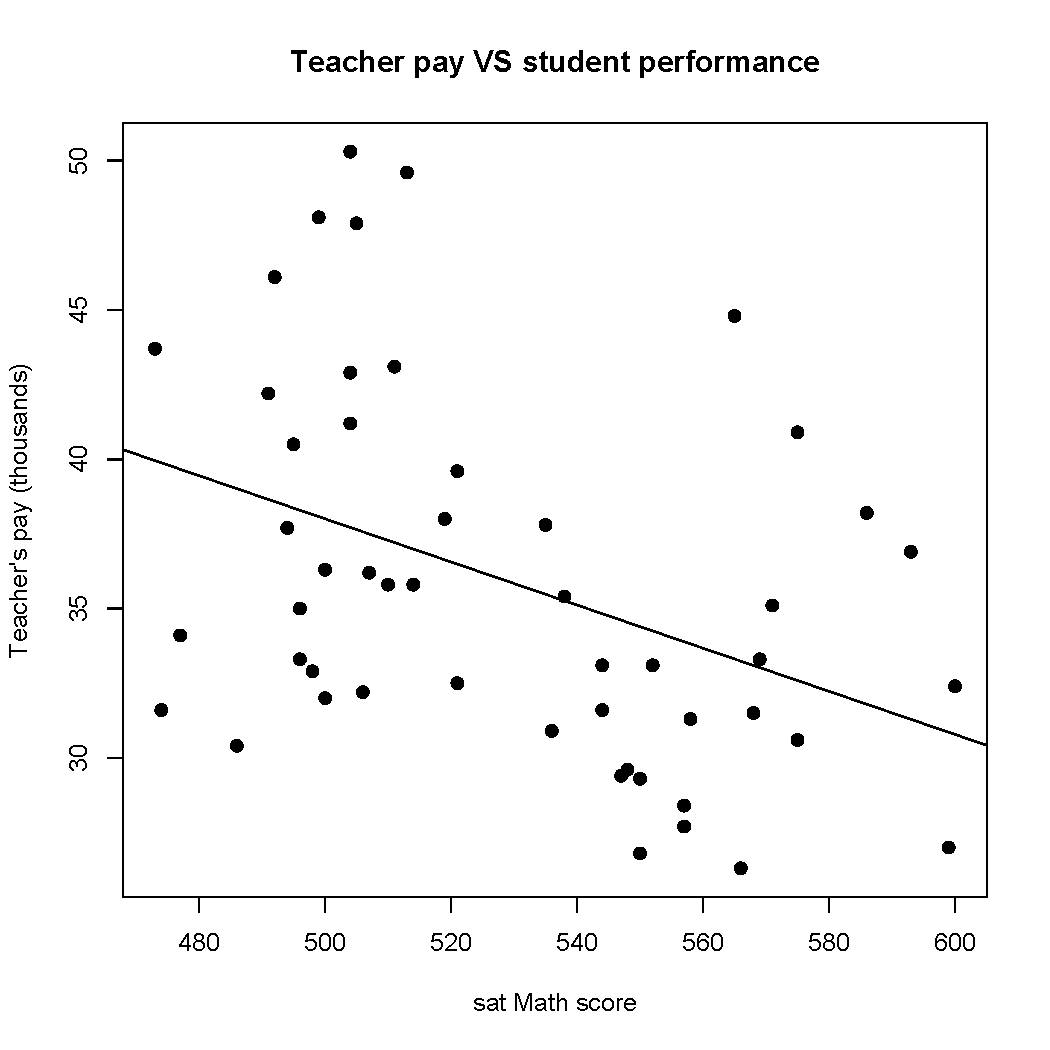
\includegraphics[width=0.7\textwidth]{/Users/biona001/Benjamin_Folder/UCLA/biomath_204/hw1/plot1.pdf}\label{fig:f1}}
  \hfill
{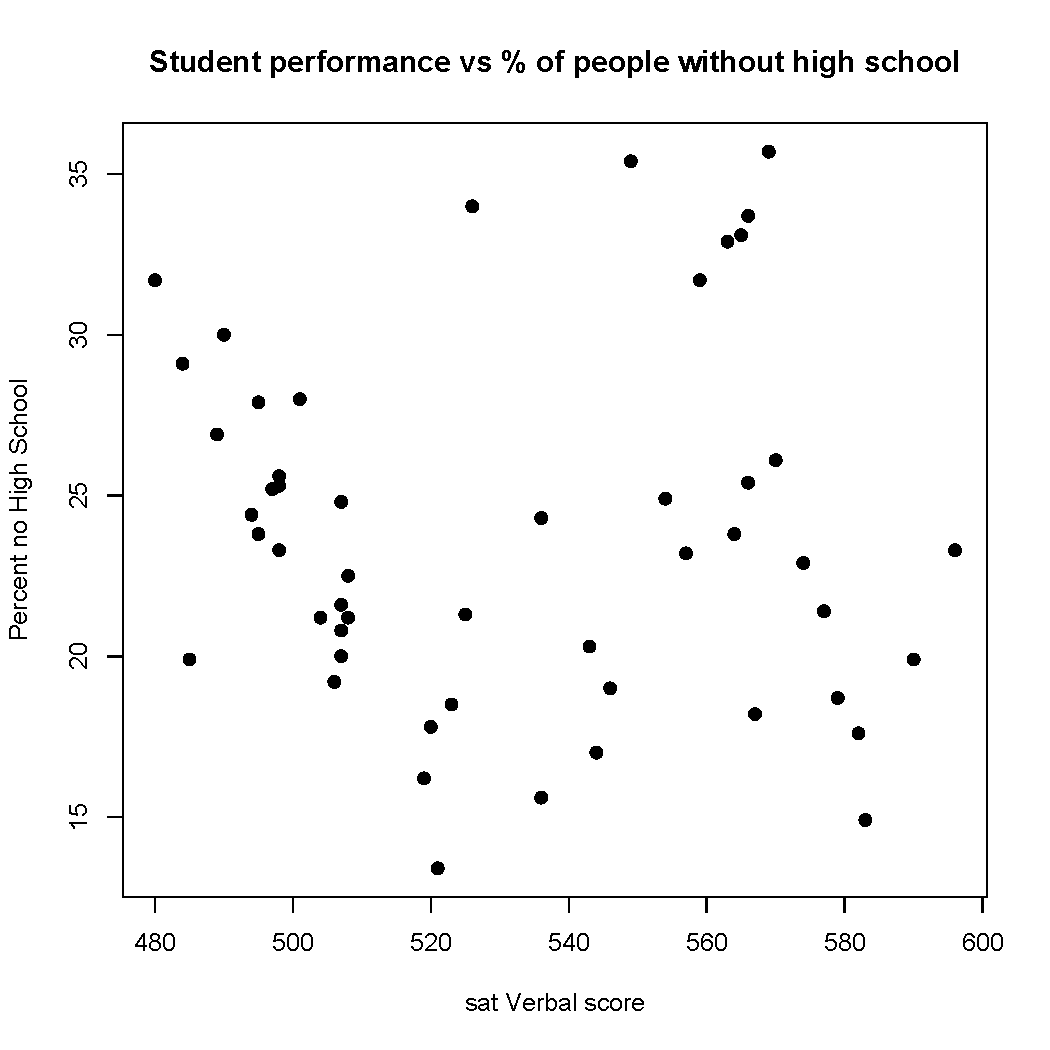
\includegraphics[width=0.7\textwidth]{/Users/biona001/Benjamin_Folder/UCLA/biomath_204/hw1/plot2.pdf}\label{fig:f2}}
\end{figure}

For the top graph, interestingly, the higher the teacher's salary the lower their student's SAT scores (i.e. these two variables have negative covariance). Intuitively we expect higher salary to reflect a higher qualification and hence teaching ability, but apparently that isn't the case. On the other hand, the bottom graph shows that while a state's population without high school education could vary considerably (from 13 to 35), that does not have any effect on student's verbal SAT score. This is another rather strange phenomenon since we would expect a more educated state to treat SAT more seriously and hence be more successful at it. \\
\\
The mode for both graph's $X$ axis is around 500. Contrary to popular beliefs, the mean is definitely not around 500. From eye inspection both graphs are obviously not normal. Finally, if we ignore the part that some states have as much as 35 percent of the population without a high school diploma, there is little unusal values. 
\end{proof}



\end{document}